\documentclass{fefu_thesis/cls/fefu}

\usepackage{float}
\usepackage{caption}
\usepackage{subcaption}

\author{Терехов Д.Е.}
\setschool{ШКОЛА ЕСТЕСТВЕННЫХ НАУК ДВФУ}
\setgroup{Б8403а}

\begin{document}
    \tableofcontents
    \pagebreak
    \begin{abstract}
        Текстурный атлас — это большое изображение, полученное склеиванием маленьких текстур. Тем самым экономится память и, что еще более важно, уменьшается количество батчей при отрисовке. В работе решается проблема полигонализации текстур и последующей упаковки в текстурные атласы.

        Упаковка текстур в текстурные атласы является частным случаем задачи об упаковке в контейнеры -- NP-трудная комбинаторная задача. Задача заключается в упаковке объектов предопределённой формы в конечное число контейнеров предопределённой формы таким способом, чтобы число использованных контейнеров было наименьшим или количество или объём объектов (которые упаковывают) были наибольшими. Для решения NP-трудной задачи были использованы методы машинного обучения.
    \end{abstract}
    \section*{Введение}
        Целью работы является разработка и внедрение алгоритмов полигонализации текстур и упаковки полигональных текстур в атласы для игровой студии <<Game Forest>>\cite{SGFSite}, которая разрабатывает игровой движок с открытым исходным кодом Citrus\cite{CitrusRepo}.

        К сожалению, эффективных алгоритмов для полигонализации и упаковки полигональных текстур в открытом доступе нет.
    \section{Глоссарий}
    \section{Первый раздел(глава)}
    \subsection{Обзор предметной области}
    \subsubsection{Студия <<Game Forest>>}
    Работа выполняется по заказу студии «Game Forest». «Game Forest» – студия
по разработке игр на мобильные устройства. Наиболее успешные проекты:
    \begin{itemize}
        \item 7 Wonders;
        \item Gummy Drop;
        \item Toy Story Drop.
    \end{itemize}
    \subsubsection{Citrus Game Engine}
    Citrus – игровой движок с открытым исходным кодом, распространяемый по лицензии GPL­3.0. репозиторий размещен на платформе Github\cite{CitrusRepo}.Citrus Game Engine состоит из следующих компонент:
    \begin{itemize}
        \item Lime -- ядро игрового движка;
        \item Lemon -- линкер сторонних библиотек;
        \item Yuzu -- библиотека для сериализации;
        \item Orange -- сборщик приложений;
        \item Tangerine -- редактор сцен;
        \item Kumquat -- генератор кода.
    \end{itemize}
    \subsubsection{Текстурный атлас}
    В компьютерной графике реального времени, текстурный атлас – это изображение, содержащее набор под­изображений, каждое из которых является текстурой для некоторого 2D или 3D объекта. Под­текстуры отображаются на объект, используя UV ­преобразование, при этом координаты в атласе задают, какую часть изображения нужно использовать. В приложениях нередко используется множество маленьких текстур, причём переключение с одной текстуры на другую является относительно медленным процессом. Поэтому в подобных ситуациях бывает целесообразно применение одного большого изображения вместо множества маленьких.
    \subsubsection{Полигонализация текстур}
    Полигонализация текстуры -- процесс обрамления текстуры в полигон и вырезание из текстуры полигональных дыр , не задевая видимые части текстуры. Сложность заключается в нахождении оптимальной полигонализации текстуры, то есть необходимо использовать наименьшее количество вершин и при этом включить в полигон наименьшее количество невидимых пикселей, так как вызов пиксельного шейдера для невидимого пикселя это бесполезная трата ресурсов видеокарты.
    \begin{figure}[H]
        \centering
        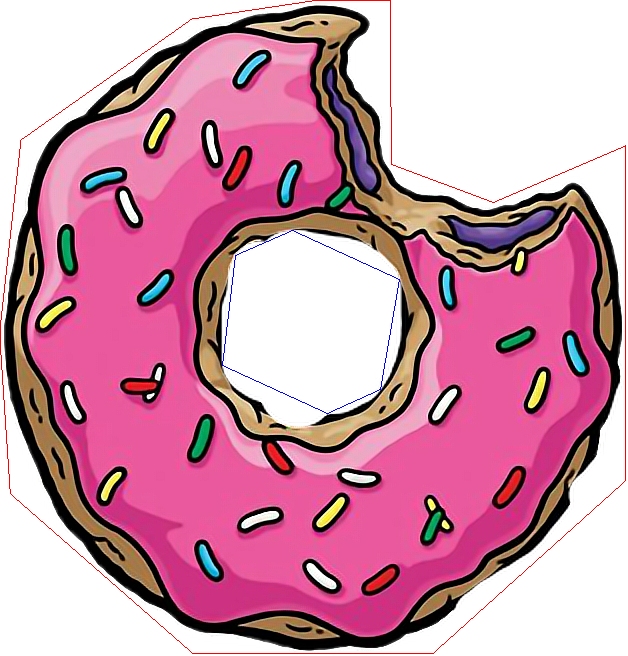
\includegraphics[scale=0.5]{images/donut_polygonized.png}
        \caption{Пример полигонизированной текстуры}
    \end{figure}
    \subsubsection{Упаковка текстур в атласы}
    Для того чтобы уменьшить количество вызовов на отрисовку текстуры пакуются в текстурные атласы. Чем меньше атласов на то же самое количество текстур, тем:
    \begin{itemize}
        \item Игра занимает меньший размер;
        \item Происходит меньше вызовов на отрисовка (меньше нагрузка на видеокарту);
        \item Меньше расходуется видеопамяти.
    \end{itemize}
    Для упаковки текстур в игровом движке Citrus используется жадный алгоритм. Текстуры пакуются прямоугольной рамкой. Полигонализация текстур способствует уменьшению занимаемой площади, а значит увеличивает плотность упаковки, уменьшает количество атласов.
    \subsection{Обзор существующих методов решения}
    Существует платный программный пакет TexturePacker\cite{TexturePacker}, который не раскрывает свои алгоритмы. Также известно о существовании внутреннего решения в компании Playrix\cite{PlayrixArticle} и в редакторе 2D анимаций Spine\cite{Spine} (однако Spine использует заготовленные пользователем полигональные сетки).

    В области bin packing problem и cutting stock problem существуют, основанные на эвристиках\cite{Heuristic1}\cite{Heuristic2}\cite{Heuristic3} или no-fit polygon\cite{NFP1}\cite{NFP2}. Также существуют работы, доказывающие эффективность генетических алгоритмов\cite{Genetica1} и particle swarm optimization (PSO)\cite{PSO1}\cite{PSO2}. Playrix в своей статье\cite{PlayrixArticle} говорят, что для упаковки текстур используют метод пчелиного роя. В некоторых статья сильно ограничивается класс фигур, например, только выпуклые или только прямоугольные. Ни в одной из статей не приводятся действительно интересные варианты упаковки со сложными фигурами, которые были бы схожи с результатами, полученными в TexturePacker. Метод no-fit polygon имеет изъян в виде ограниченного количества ориентаций полигона. Примеры из статей, использующих PSO, работают медленно и не могут быть использованы для сборки игры.

    Было решено создать собственное решение, которые отвечало бы следующим требованиям:
    \begin{itemize}
        \item Класс фигур ограничивается простыми полигонами с дырками (т.е. не подходят только полигоны, имеющие самопересечения. Такие полигоны необходимо разделить на несколько простых на этапе препроцессинга);
        \item Время упаковки не должно <<слишком сильно>> увеличиться.
    \end{itemize}
    \section{Второй раздел(глава)}
    Блаблабла
    \subsection{Выделение контура}
    Алгоритмы выделения контура можно разделить на 3 типа: обход попиксельно, обход повершинно, run-data.
    \subsubsection{Обход попиксельно}
    Метод выделения контура обходом попиксельно начинает с какого-либо стартового пикселя и пиксель за пикселем обходит контур изображения предопределенным образом, а затем сохраняет их координаты в памяти в соответствии с порядком трассировки. Наиболее известные алгоритмы обхода контура попиксельно: Moore-neighbor tracing\cite{MoorNeighbor}, radial sweep\cite{RadialSweep} и алгоритм Theo Pavlidis\cite{TheoPavlidis}.
    \subsubsection{Обход повершинно}
    Метод выделения контура обходом повершинно отличается от обхода попиксельно лишь тем, что обход осуществляется по границам пикселя.
    \subsubsection{Run-data}
    Run-data методы выделения контура проходят по изображению сканирующей линией оставляя определенные метки на встреченном граничном пикселе. Далее по расставленным меткам восстанавливается контур изображения. Примеры методов этой группы: run-type direction code, методы, основанные на PXY таблицы. Отличительной особенностью run-data методов является возможность выделения внешних и внутренних контуров, сохраняя иерархию. Так же способ обхода изображения в некоторых алгоритмах позволяет не держать в памяти изображение целиком.

    Было решено выбрать алгоритм именно из этой группы методов, так как по заданию необходимо выделять дырки на объектах. Выбор пал на алгоритм Suzuki Satoshi \cite{SuzukiAlgorithm}, использующийся в библиотеке OpenCV. Он достаточно прост в реализации, умеет иерархически выделять контуры. Псевдокод выбранного алгоритма приведен ниже:
    \subsection{Полигонизация}
    В области полигонизации текстур нет известных алгоритмов, однако в области картографии используются алгоритмы упрощения кривой (на карте с помощью их упрощается береговая линия при отдалении камеры). Самыми известными алгоритмами в этой области являются алгоритмы Visvalingam–Whyatt\cite{VisvalingamWhyatt} и Ramer–Douglas–Peucker\cite{DouglasPeucker}. Из этих алгоритмов были взяты некоторые идеи.

    \subsubsection{Неформальное описание алгоритма}
        \begin{enumerate}
            \item Выделить иерархический контур текстуры
            \item Рассчитать минимальное (по отсекаемой площади) возможную трансформацию для каждой вершины.
            \item Пока условие выхода не достигнуто и существует минимальная возможная трансформация, то необходимо применить её и исключить из рассмотрения.
            \item Если минимальная возможная трансформация не существует, то необходимо смерджить 2 полигона таким образом, чтобы удаленных вершин и захваченных прозрачных пикселей было минимальным, и вернуться к шагу 3.
            \item Если не существует полигонов, которые можно было бы смерджить, то необходимо удалить полигон-дырку так, чтобы количество удаленных вершин и захваченных прозрачных пикселей было минимальным, и вернуться к шагу 3.
            \item К этому моменты должен остаться один полигон-граница. Необходимо спроецировать точки полигона таким образом, чтобы можно было появилось хотя бы одно минимальное возможное преобразование, и вернуться к шагу три. В противном случае мы достигли либо ббокса изображения либо объемлющего треугольника.
        \end{enumerate}

    \subsubsection{Преобразования}
        \begin{enumerate}
            \item Удаление вогнутого угла для границы или выпуклого для дырки;
            \item Замена вершины пересечением двух сторон;
            \item Удаление треугольной дырки.
        \end{enumerate}
        \begin{figure}[H]
            \centering
            \begin{subfigure}[H]{\linewidth}
                \centering
                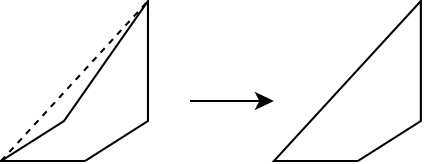
\includegraphics[scale=2]{images/convex_angle.png}
                \caption{Удаление вогнутого угла}
            \end{subfigure}
            \vskip .5cm
            \begin{subfigure}[H]{\linewidth}
                \centering
                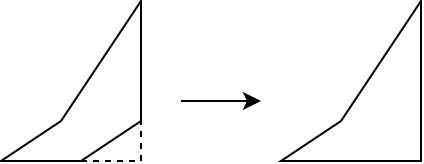
\includegraphics[scale=2]{images/sides_intersection.png}
                \caption{Пересечение 2 сторон}
            \end{subfigure}
        \end{figure}
    \subsubsection{Бэкэнд для операций}
    Для проверки преобразований и их выполнения используется триангуляция Делоне\cite{Delaunay} из бакалаврской работы, также сделанной по заказу студии <<Game Forest>> . Жесткими ребрами задаются границы полигонов. Операцией вставки структурных ребер проверяется возможность преобразования. Преобразования применяются при помощи операций вставки и удаления вершин, а также вставки структурных ребер. Данный подход позволил сильно снизить время на разработку и отладку сложного математического кода, для которого было бы сложнее добиться нужной асимптотики.
    \subsection{Упаковка}
    Генетический алгоритм с локальным поиском (memetic algorithm). Методы локального поиска:
    \begin{itemize}
        \item Вставить полигон в пустое место
        \item Вставить полигон в дырку
        \item Физика
    \end{itemize}
    \section{Третий раздел(глава)}
    \section{Заключение}
    \newpage
    \bibliographystyle{ugost2008ls}
    \bibliography{references}
\end{document}
